\documentclass{beamer}

% Required packages
\usepackage{amsmath}
\usepackage{physics}
\usepackage{graphicx}
\usepackage{siunitx}
\usepackage{xcolor}

% Set image search paths
\graphicspath{{../images/}{../../shared/images/}}

% Define custom colors for DS9 theme
\definecolor{ds9blue}{RGB}{25,25,112}
\definecolor{ds9gold}{RGB}{218,165,32}
\definecolor{ds9grey}{RGB}{105,105,105}
\definecolor{ds9red}{RGB}{178,34,34}

% Set up the Madrid theme with custom colors
\usetheme{Madrid}
\usecolortheme{whale}

\setbeamercolor{palette primary}{bg=ds9blue,fg=white}
\setbeamercolor{palette secondary}{bg=ds9grey,fg=white}
\setbeamercolor{palette tertiary}{bg=ds9gold,fg=black}
\setbeamercolor{palette quaternary}{bg=ds9red,fg=white}
\setbeamercolor{structure}{fg=ds9blue}
\setbeamercolor{title}{fg=ds9gold}
\setbeamercolor{subtitle}{fg=ds9gold}
\setbeamercolor{frametitle}{bg=ds9blue,fg=white}
\setbeamercolor{block title}{bg=ds9blue,fg=white}
\setbeamercolor{block body}{bg=ds9grey!20,fg=black}

% Title page configuration
\title[Electric Circuits]{PHYS12 CH: 20, 21}
\subtitle{Electric Circuits: Principles, Applications, and Safety}
\author[Mr. Gullo]{Mr. Gullo}
\date[Apr 2025]{April 8, 2025}
\institute[Physics Dept.]{Physics Department}

\begin{document}

% Title page
\begin{frame}
    \titlepage
\end{frame}

% Table of contents
\begin{frame}
    \frametitle{Lesson Overview}
    \tableofcontents
\end{frame}

% Learning objectives
\section{Introduction}
\begin{frame}
    \frametitle{Learning Objectives}
    \begin{block}{By the end of this lesson, you will be able to:}
        \begin{itemize}
            \item Define current, resistance, and voltage and explain their relationships
            \item Apply Ohm's law to simple circuits
            \item Calculate equivalent resistance for series and parallel circuits
            \item Calculate electric power and energy in circuits
            \item Distinguish between AC and DC circuits and their properties
            \item Describe electric hazards and bioelectrical applications
            \item Explain how measuring instruments work in DC circuits
            \item Understand null measurement techniques
            \item Describe the behavior of RC circuits during charging and discharging
            \item Solve complex circuit problems using Kirchhoff's rules
        \end{itemize}
    \end{block}
\end{frame}

% Current and Ohm's Law section
\section{Current and Ohm's Law}
\begin{frame}
    \frametitle{Electric Current}
    \begin{block}{Definition}
        Electric current is the rate at which charge flows:
        \[ I = \frac{\Delta Q}{\Delta t} \]
        where $\Delta Q$ is the amount of charge passing through an area in time $\Delta t$.
    \end{block}
    \begin{itemize}
        \item SI unit: ampere (A), where 1 A = 1 C/s
        \item Conventional current: direction of positive charge movement
        \item Current is the flow of free charges (electrons, ions)
        \item Related to drift velocity: $I = nqAv_d$
    \end{itemize}
    \end{frame}
    \begin{frame}{}
    \begin{figure}
        \centering
        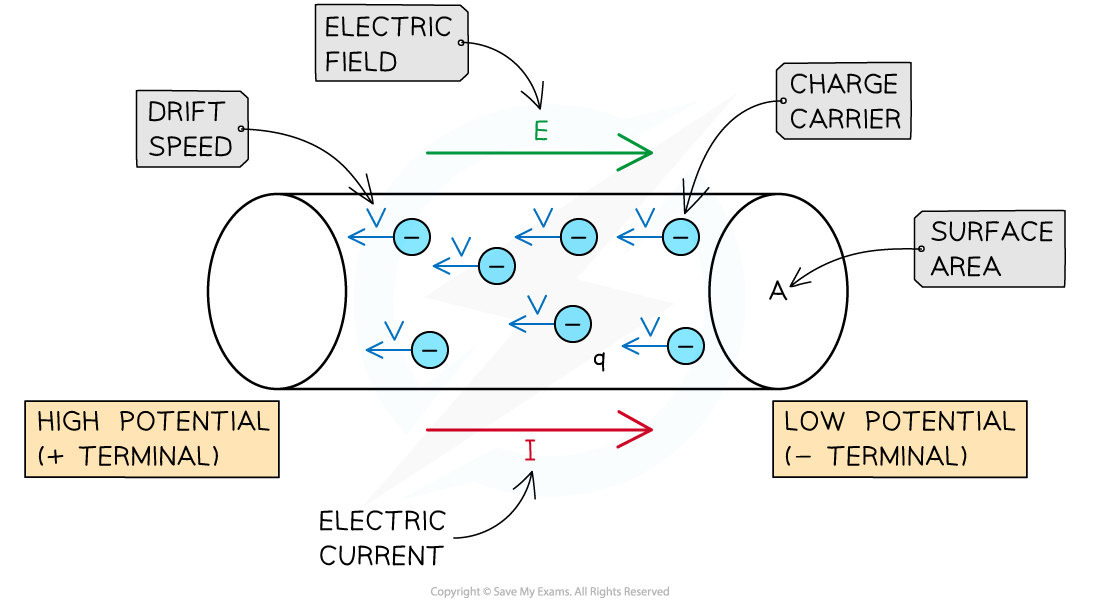
\includegraphics[width=1\linewidth]{5-1-2-charge-carriers-drifting-along-the-conductor_sl-physics-rn-3.png}
    \end{figure}
\end{frame}

\begin{frame}
    \frametitle{Ohm's Law and Simple Circuits}
    \begin{block}{Ohm's Law}
        For a simple circuit with a single voltage source and resistance:
        \[ I = \frac{V}{R} \]
    \end{block}
    \begin{itemize}
        \item Resistance ($R$): opposition to current flow
        \item Unit: ohm ($\Omega$), where 1 $\Omega$ = 1 V/A
        \item Voltage drop across a resistor: $V = IR$
    \end{itemize}
    \begin{center}
        \begin{figure}
            \centering
            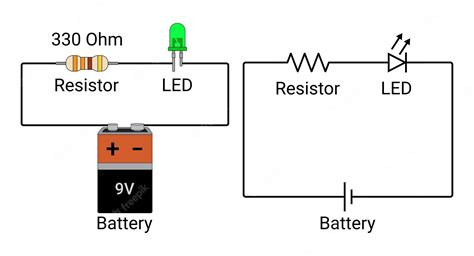
\includegraphics[width=0.5\linewidth]{th-991058791.jpg}
        \end{figure}
    \end{center}
\end{frame}

\begin{frame}
    \frametitle{Resistance and Resistivity}
    \begin{block}{Resistance Formula}
        For a cylindrical conductor:
        \[ R = \rho\frac{L}{A} \]
        where $\rho$ is resistivity, $L$ is length, and $A$ is cross-sectional area.
    \end{block}
    \begin{itemize}
        \item Materials classified as conductors, semiconductors, or insulators
        \item Temperature affects resistivity: $\rho = \rho_0(1 + \alpha\Delta T)$
        \item Temperature affects resistance: $R = R_0(1 + \alpha\Delta T)$
        \item $\alpha$ is the temperature coefficient of resistivity
    \end{itemize}
\end{frame}
\begin{frame}{}
    \begin{figure}
        \centering
        
\includegraphics[width=1\linewidth]{image.png}
    \end{figure}
\end{frame}

\begin{frame}
    \frametitle{Electric Power and Energy}
    \begin{block}{Electric Power}
        Rate at which electrical energy is supplied or dissipated:
        \[ P = IV = \frac{V^2}{R} = I^2R \]
    \end{block}
    \begin{itemize}
        \item Energy used: $E = Pt$
        \item Units: Watts (W) for power, Joules (J) for energy
        \item Example: A 60W light bulb connected to 120V draws 0.5A
    \end{itemize}
    \vspace{0.5cm}
    \begin{alertblock}{Power Comparison}
        Different power ratings lead to different brightness in bulbs,
        different amounts of heat generated in resistors, etc.
    \end{alertblock}
\end{frame}

\begin{frame}
    \frametitle{AC vs. DC}
    \begin{block}{Direct Current (DC)}
        \begin{itemize}
            \item Current flows in only one direction
            \item Source voltage is constant
            \item Examples: batteries, solar cells, DC power supplies
        \end{itemize}
    \end{block}
    \begin{block}{Alternating Current (AC)}
        \begin{itemize}
            \item Voltage varies sinusoidally: $V = V_0 \sin 2\pi ft$
            \item Current varies sinusoidally: $I = I_0 \sin 2\pi ft$
            \item $V_0$ and $I_0$ are peak values, $f$ is frequency in Hz
            \item Examples: household electricity, power transmission
        \end{itemize}
    \end{block}
\end{frame}

\begin{frame}
    \frametitle{AC Power and RMS Values}
    \begin{block}{Average AC Power}
        \[ P_{ave} = \frac{1}{2}I_0V_0 = I_{rms}V_{rms} \]
    \end{block}
    \begin{itemize}
        \item RMS (Root Mean Square) values:
        \[ I_{rms} = \frac{I_0}{\sqrt{2}} \quad \text{and} \quad V_{rms} = \frac{V_0}{\sqrt{2}} \]
        \item Ohm's Law for AC: $I_{rms} = \frac{V_{rms}}{R}$
        \item Power formulas (similar to DC):
        \[ P_{ave} = I_{rms}V_{rms} = \frac{V_{rms}^2}{R} = I_{rms}^2R \]
    \end{itemize}
  \end{frame}

\begin{frame}
\begin{figure}
      \centering
      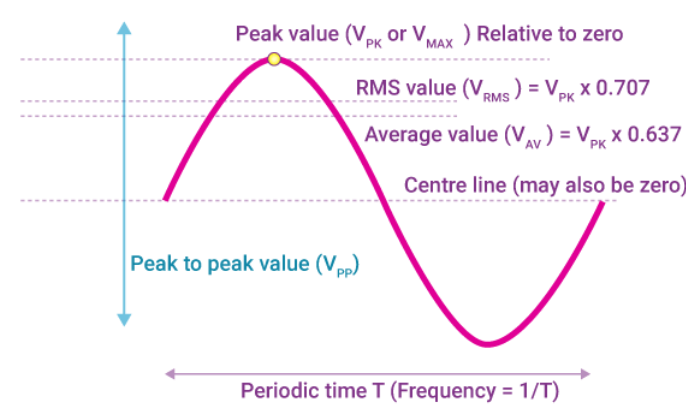
\includegraphics[width=0.75\linewidth]{rms.png}
  \end{figure}
\end{frame}

\begin{frame}
    \frametitle{Electric Hazards and the Human Body}
    \begin{block}{Types of Electric Hazards}
        \begin{itemize}
            \item Thermal hazards: Excessive power causing burns or fires
            \item Shock hazards: Current flowing through a person
        \end{itemize}
    \end{block}
    \begin{block}{Shock Severity Factors}
        \begin{itemize}
            \item Current magnitude
            \item Current path through body
            \item Duration of exposure
            \item AC frequency
        \end{itemize}
    \end{block}
    \begin{center}
        \begin{tabular}{|c|l|}
            \hline
            \textbf{Current (mA)} & \textbf{Effect on Human Body} \\
            \hline
            1 & Threshold of perception \\
            5 & Painful shock, can cause muscle contraction \\
            10-20 & Cannot let go, respiratory paralysis \\
            100-300 & Ventricular fibrillation, potential death \\
            \hline
        \end{tabular}
    \end{center}
\end{frame}

\begin{frame}
    \frametitle{Nerve Conduction and Bioelectricity}
    \begin{block}{Bioelectricity Basics}
        \begin{itemize}
            \item Electric potentials in neurons created by ionic concentration differences
            \item Semipermeable membranes separate different ionic concentrations
            \item Stimuli change membrane permeability, creating action potentials
            \item Action potentials propagate along neurons as electrical signals
        \end{itemize}
    \end{block}
    \begin{block}{Electrocardiogram (ECG)}
        \begin{itemize}
            \item Records electrical activity of the heart
            \item Measures voltage differences on body surface
            \item Helps diagnose heart conditions and abnormalities
        \end{itemize}
    \end{block}
   
\end{frame}
\begin{frame}{}
    \begin{figure}
        \centering
        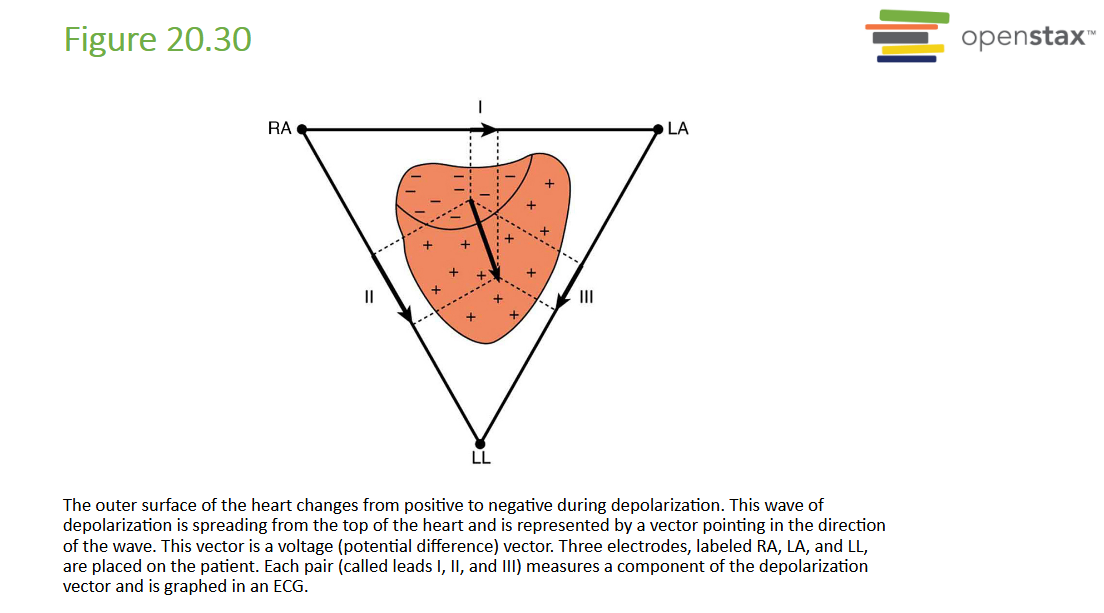
\includegraphics[width=1\linewidth]{ecg.png}
    \end{figure}
\end{frame}

% Complex Circuits section
\section{Complex Circuits}
\begin{frame}
    \frametitle{Resistors in Series}
    \begin{block}{Series Configuration}
        Resistors are in series when they are connected end-to-end.
        \[ R_s = R_1 + R_2 + R_3 + \ldots \]
    \end{block}
    \begin{itemize}
        \item Same current flows through each resistor
        \item Voltage is divided among resistors: $V = V_1 + V_2 + V_3 + \ldots$
        \item Individual voltage drops: $V_1 = IR_1$, $V_2 = IR_2$, etc.
    \end{itemize}
    \begin{center}
       \begin{figure}
           \centering
           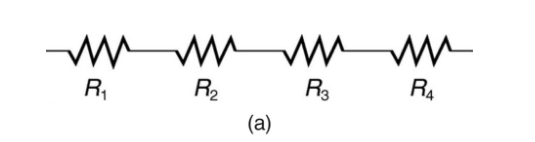
\includegraphics[width=0.75\linewidth]{serres.png}
       \end{figure}
    \end{center}
\end{frame}

\begin{frame}
    \frametitle{Resistors in Parallel}
    \begin{block}{Parallel Configuration}
        Resistors are in parallel when they share the same two endpoints.
        \[ \frac{1}{R_p} = \frac{1}{R_1} + \frac{1}{R_2} + \frac{1}{R_3} + \ldots \]
    \end{block}
    \begin{itemize}
        \item Same voltage across each resistor
        \item Current divides among resistors: $I = I_1 + I_2 + I_3 + \ldots$
        \item Individual currents: $I_1 = \frac{V}{R_1}$, $I_2 = \frac{V}{R_2}$, etc.
    \end{itemize}
    \begin{center}
        \begin{figure}
            \centering
            
\includegraphics[width=0.5\linewidth]{image.png}
        \end{figure}
    \end{center}
\end{frame}

\begin{frame}
    \frametitle{Electromotive Force and Terminal Voltage}
    \begin{block}{Voltage Source Components}
        A real voltage source has:
        \begin{itemize}
            \item Electromotive force (emf): potential difference when no current flows
            \item Internal resistance ($r$): resistance within the source
        \end{itemize}
    \end{block}
    \begin{itemize}
        \item Terminal voltage: $V = \text{emf} - Ir$
        \item Series voltage sources: internal resistances add, emfs add algebraically
        \item Solar cells: series for increased voltage, parallel for increased current
    \end{itemize}
    
\end{frame}
\begin{frame}
\begin{figure}
    \centering
    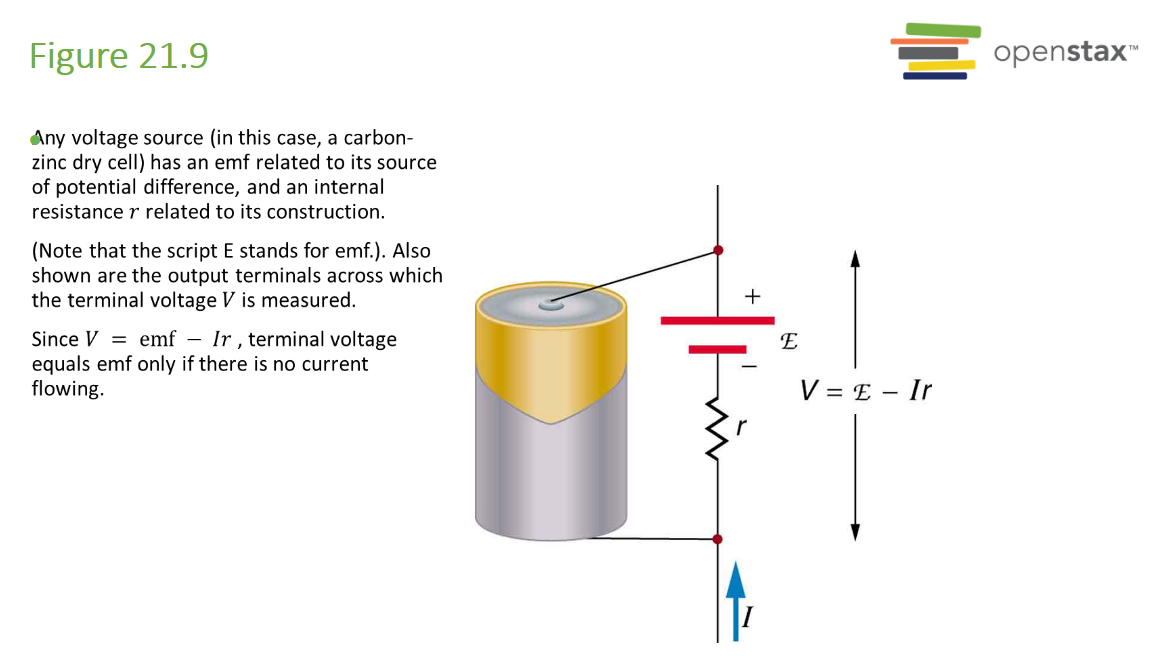
\includegraphics[width=1\linewidth]{inres.png}
\end{figure}
\end{frame}
\begin{frame}
    \frametitle{Kirchhoff's Rules}
    \begin{block}{Junction Rule (First Rule)}
        The sum of all currents entering a junction must equal the sum of all currents leaving the junction.
        \[ \sum I_{\text{in}} = \sum I_{\text{out}} \]
    \end{block}
    \begin{block}{Loop Rule (Second Rule)}
        The algebraic sum of potential changes around any closed circuit path (loop) must be zero.
        \[ \sum \Delta V = 0 \]
    \end{block}
    \begin{itemize}
        \item Based on conservation of charge and energy
        \item Essential for analyzing complex circuits
    \end{itemize}
    \end{frame}
    \begin{frame}{}
       
    \begin{figure}
        \centering
        \includegraphics[width=1\linewidth]{junctionloopkirchov.jpg}
    \end{figure}
\end{frame}

\begin{frame}
    \frametitle{DC Voltmeters and Ammeters}
    \begin{block}{Measuring Instruments}
        \begin{itemize}
            \item Voltmeters measure voltage (potential difference)
            \item Ammeters measure current
        \end{itemize}
    \end{block}
    \begin{columns}
        \begin{column}{0.5\textwidth}
            \textbf{Voltmeter Characteristics:}
            \begin{itemize}
                \item Connected in parallel with component
                \item Must have very high resistance
                \item Minimizes impact on circuit
            \end{itemize}
        \end{column}
        \begin{column}{0.5\textwidth}
            \textbf{Ammeter Characteristics:}
            \begin{itemize}
                \item Connected in series with circuit
                \item Must have very low resistance
                \item Minimizes voltage drop
            \end{itemize}
        \end{column}
    \end{columns}
    \begin{figure}
        \centering
        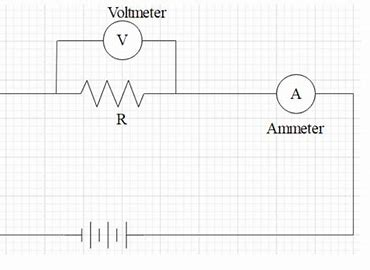
\includegraphics[width=0.3\linewidth]{amvolmm.jpg}
    \end{figure}
\end{frame}

\begin{frame}
    \frametitle{Null Measurements}
    \begin{block}{Null Measurement Technique}
        \begin{itemize}
            \item Achieves greater accuracy by balancing a circuit
            \item No current flows through measuring device at balance point
            \item Used for precise voltage and resistance measurements
        \end{itemize}
    \end{block}
    \begin{columns}
        \begin{column}{0.5\textwidth}
            \textbf{Potentiometer:}
            \begin{itemize}
                \item Determines voltage precisely
                \item Uses a calibrated variable resistance
                \item Balances unknown voltage against known voltage
            \end{itemize}
        \end{column}
        \begin{column}{0.5\textwidth}
            \textbf{Wheatstone Bridge:}
            \begin{itemize}
                \item Determines resistance precisely
                \item Uses ratio of resistances
                \item At balance: $\frac{R_1}{R_2} = \frac{R_x}{R_3}$
            \end{itemize}
   
    \begin{figure}
        \centering
        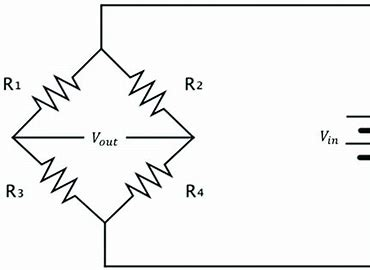
\includegraphics[width=0.5\linewidth]{wheatstone.jpg}
    \end{figure}
         \end{column}
    \end{columns}
\end{frame}

% RC Circuits section
\section{RC Circuits}
\begin{frame}
    \frametitle{RC Circuits Basics}
    \begin{block}{RC Circuit Definition}
        A circuit containing both a resistor and a capacitor.
    \end{block}
    \begin{itemize}
        \item Time constant: $\tau = RC$
        \item Determines the rate of charging or discharging
        \item Units: seconds (s)
    \end{itemize}
   
        \begin{figure}
            \centering
            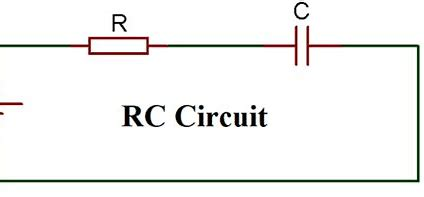
\includegraphics[width=0.65\linewidth]{OIP-C.jpg}
        \end{figure}
  
\end{frame}

\begin{frame}
    \frametitle{Charging and Discharging RC Circuits}
    \begin{block}{Charging a Capacitor}
        When an initially uncharged capacitor ($V_0 = 0$ at $t = 0$) is charged:
        \[ V = \text{emf}(1-e^{-t/RC}) \]
    \end{block}
    \begin{block}{Discharging a Capacitor}
        When a capacitor with initial voltage $V_0$ is discharged:
        \[ V = V_0e^{-t/RC} \]
    \end{block}
    \begin{itemize}
        \item Charging: voltage rises by 0.632 of remaining value per time constant
        \item Discharging: voltage falls by 0.368 of remaining value per time constant
    \end{itemize}
\end{frame}

\begin{frame}
    \frametitle{RC Circuits: Graphical Representation}
    \begin{center}
        \begin{tabular}{cc}
            \begin{figure}
    \centering
    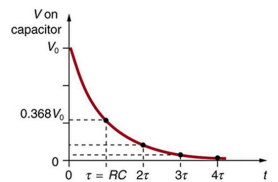
\includegraphics[width=0.5\linewidth]{dischcurve.png}
\end{figure} 
&
\begin{figure}
                \centering
                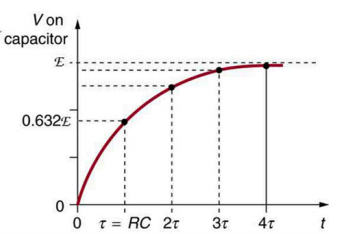
\includegraphics[width=0.4\linewidth]{charge.png}
            \end{figure} \\


                        Charging: $V = \text{emf}(1-e^{-t/RC})$ & Discharging: $V = V_0e^{-t/RC}$
        \end{tabular}
    \end{center}
    \begin{itemize}
        \item Both processes are asymptotic
        \item Full charging/discharging theoretically takes infinite time
        \item Practically complete (99.99\%) after 5 time constants
    \end{itemize}
\end{frame}

% Examples section
\section{Examples}
\begin{frame}
    \frametitle{I Do: Equivalent Resistance Calculation}
    \begin{block}{Problem}
        Calculate the equivalent resistance of a circuit with three resistors: $R_1 = 2.0~\Omega$ and $R_2 = 4.0~\Omega$ in parallel, and $R_3 = 3.0~\Omega$ in series with the parallel combination.
    \end{block}
    \begin{block}{Solution}
        Step 1: Find the equivalent resistance of $R_1$ and $R_2$ in parallel.
        \begin{align*}
            \frac{1}{R_p} &= \frac{1}{R_1} + \frac{1}{R_2} = \frac{1}{2.0~\Omega} + \frac{1}{4.0~\Omega}\\
            &= 0.5~\Omega^{-1} + 0.25~\Omega^{-1} = 0.75~\Omega^{-1}\\
            R_p &= \frac{1}{0.75~\Omega^{-1}} = 1.33~\Omega
        \end{align*}
        
        Step 2: Find the total resistance by adding $R_p$ and $R_3$ in series.
        \begin{align*}
            R_{total} &= R_p + R_3 = 1.33~\Omega + 3.0~\Omega = 4.33~\Omega
        \end{align*}
    \end{block}
\end{frame}

\begin{frame}
    \frametitle{We Do: Current and Power in a Parallel Circuit}
    \begin{block}{Problem}
        For the circuit shown with a 12V battery, $R_1 = 4\Omega$ and $R_2 = 8\Omega$ in parallel, calculate:
        \begin{enumerate}[(a)]
            \item The equivalent resistance
            \item The total current from the battery
            \item The current through each resistor
            \item The voltage across each resistor
            \item The power dissipated by each resistor
        \end{enumerate}
    \end{block}
    \begin{figure}
        \centering
        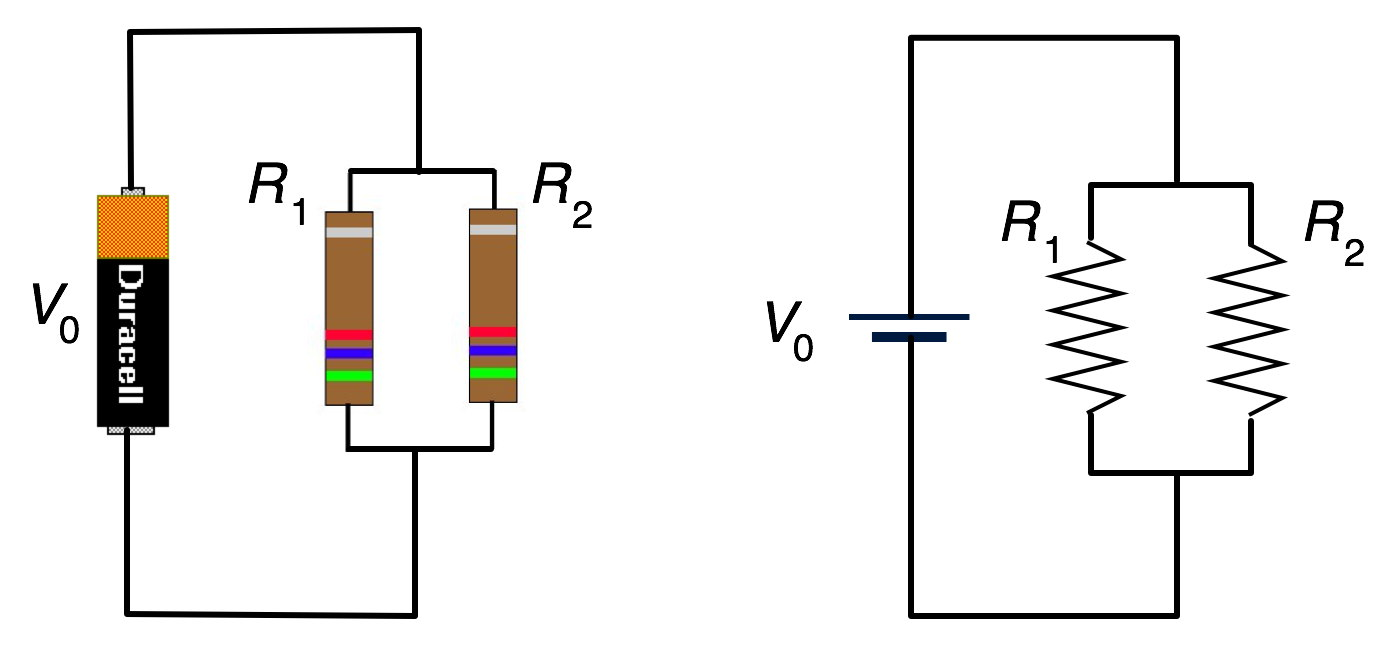
\includegraphics[width=0.5\linewidth]{ParallelCircuitbat.jpg}
    \end{figure}
\end{frame}

\begin{frame}
    \frametitle{We Do: Current and Power in a Parallel Circuit}
    \begin{block}{Partial Solution}
        (a) Equivalent resistance:
        \begin{align*}
            \frac{1}{R_{eq}} &= \frac{1}{R_1} + \frac{1}{R_2} = \frac{1}{4\Omega} + \frac{1}{8\Omega}\\
            &= 0.25\Omega^{-1} + 0.125\Omega^{-1} = 0.375\Omega^{-1}\\
            R_{eq} &= \frac{1}{0.375\Omega^{-1}} = 2.67\Omega
        \end{align*}
        
        (b) Total current from the battery:
        \begin{align*}
            I_{total} &= \frac{V}{R_{eq}} = \frac{12V}{2.67\Omega} = 4.5A
        \end{align*}
        
        (c) Current through each resistor:
        \begin{align*}
            I_1 &= \frac{V}{R_1} = \frac{12V}{4\Omega} = 3A\\
            I_2 &= \text{?} \quad \text{(complete this step)}
        \end{align*}
    \end{block}
\end{frame}

\begin{frame}
    \frametitle{We Do: Current and Power in a Parallel Circuit}
    \begin{block}{Partial Solution (cont.)}
        (d) Voltage across each resistor:
        \begin{align*}
            V_1 &= \text{?} \quad \text{(complete this step)}\\
            V_2 &= \text{?} \quad \text{(complete this step)}
        \end{align*}
        
        (e) Power dissipated by each resistor:
        \begin{align*}
            P_1 &= \text{?} \quad \text{(complete this step)}\\
            P_2 &= \text{?} \quad \text{(complete this step)}
        \end{align*}
    \end{block}
\end{frame}

\begin{frame}
    \frametitle{You Do: Terminal Voltage and Power}
    \begin{block}{Problem}
        A circuit contains a 9V battery with internal resistance $r = 0.5\Omega$ connected to a resistor $R = 5.5\Omega$.
        \begin{enumerate}[(a)]
            \item Calculate the terminal voltage.
            \item Calculate the current in the circuit.
            \item Calculate the power dissipated in the resistor.
            \item Calculate the power dissipated in the battery's internal resistance.
            \item Calculate the power supplied by the battery's emf.
        \end{enumerate}
    \end{block}
    \end{frame}

% Summary section
\section{Summary}
\begin{frame}
    \frametitle{Key Equations}
    \begin{columns}
        \begin{column}{0.5\textwidth}
            \textbf{Current and Resistance:}
            \begin{itemize}
                \item $I = \frac{\Delta Q}{\Delta t}$
                \item $I = \frac{V}{R}$ (Ohm's Law)
                \item $R = \rho\frac{L}{A}$
            \end{itemize}
            
            \textbf{Power and Energy:}
            \begin{itemize}
                \item $P = IV = \frac{V^2}{R} = I^2R$
                \item $E = Pt$
            \end{itemize}
            
            \textbf{AC Circuits:}
            \begin{itemize}
                \item $V = V_0 \sin 2\pi ft$
                \item $I_{rms} = \frac{I_0}{\sqrt{2}}$
                \item $V_{rms} = \frac{V_0}{\sqrt{2}}$
            \end{itemize}
        \end{column}
        \begin{column}{0.5\textwidth}
            \textbf{Circuit Analysis:}
            \begin{itemize}
                \item $R_s = R_1 + R_2 + R_3 + \ldots$
                \item $\frac{1}{R_p} = \frac{1}{R_1} + \frac{1}{R_2} + \ldots$
                \item $V = \text{emf} - Ir$
                \item $\sum I_{\text{in}} = \sum I_{\text{out}}$
                \item $\sum \Delta V = 0$
            \end{itemize}
            
            \textbf{RC Circuits:}
            \begin{itemize}
                \item $\tau = RC$
                \item $V = \text{emf}(1-e^{-t/RC})$ (charging)
                \item $V = V_0e^{-t/RC}$ (discharging)
            \end{itemize}
            
            \textbf{Null Measurements:}
            \begin{itemize}
                \item $\frac{R_1}{R_2} = \frac{R_x}{R_3}$ (Wheatstone bridge)
            \end{itemize}
        \end{column}
    \end{columns}
\end{frame}

\begin{frame}
    \frametitle{Concept Review}
    \begin{itemize}
        \item Current is the rate of charge flow; resistance opposes current.
        \item Ohm's Law relates current, voltage, and resistance in simple circuits.
        \item Power measures the rate of energy transfer in circuits.
        \item DC provides constant voltage; AC varies sinusoidally with time.
        \item Series resistance increases; parallel resistance decreases.
        \item Real voltage sources have internal resistance that affects terminal voltage.
        \item Kirchhoff's rules help analyze complex circuits using conservation principles.
        \item Proper measuring instrument connection is crucial for accurate readings.
        \item Null measurement techniques provide greater accuracy for precise measurements.
        \item RC circuits show exponential charging and discharging behavior characterized by the time constant $\tau$.
        \item Electrical safety requires understanding current thresholds and shock hazards.
    \end{itemize}
\end{frame}

\begin{frame}
    \frametitle{Questions?}
    \begin{center}
        \Large Thank you for your attention!
        
        \vspace{1cm}
        
        Any questions?
    \end{center}
\end{frame}

\end{document}